\section{Frequency mode 08}
\label{FM08}

\subsection{Spectra}
\label{FM08:spectra}

\begin{figure}[ht]
    \centering
    \begin{subfigure}[b]{0.9545\textwidth}
        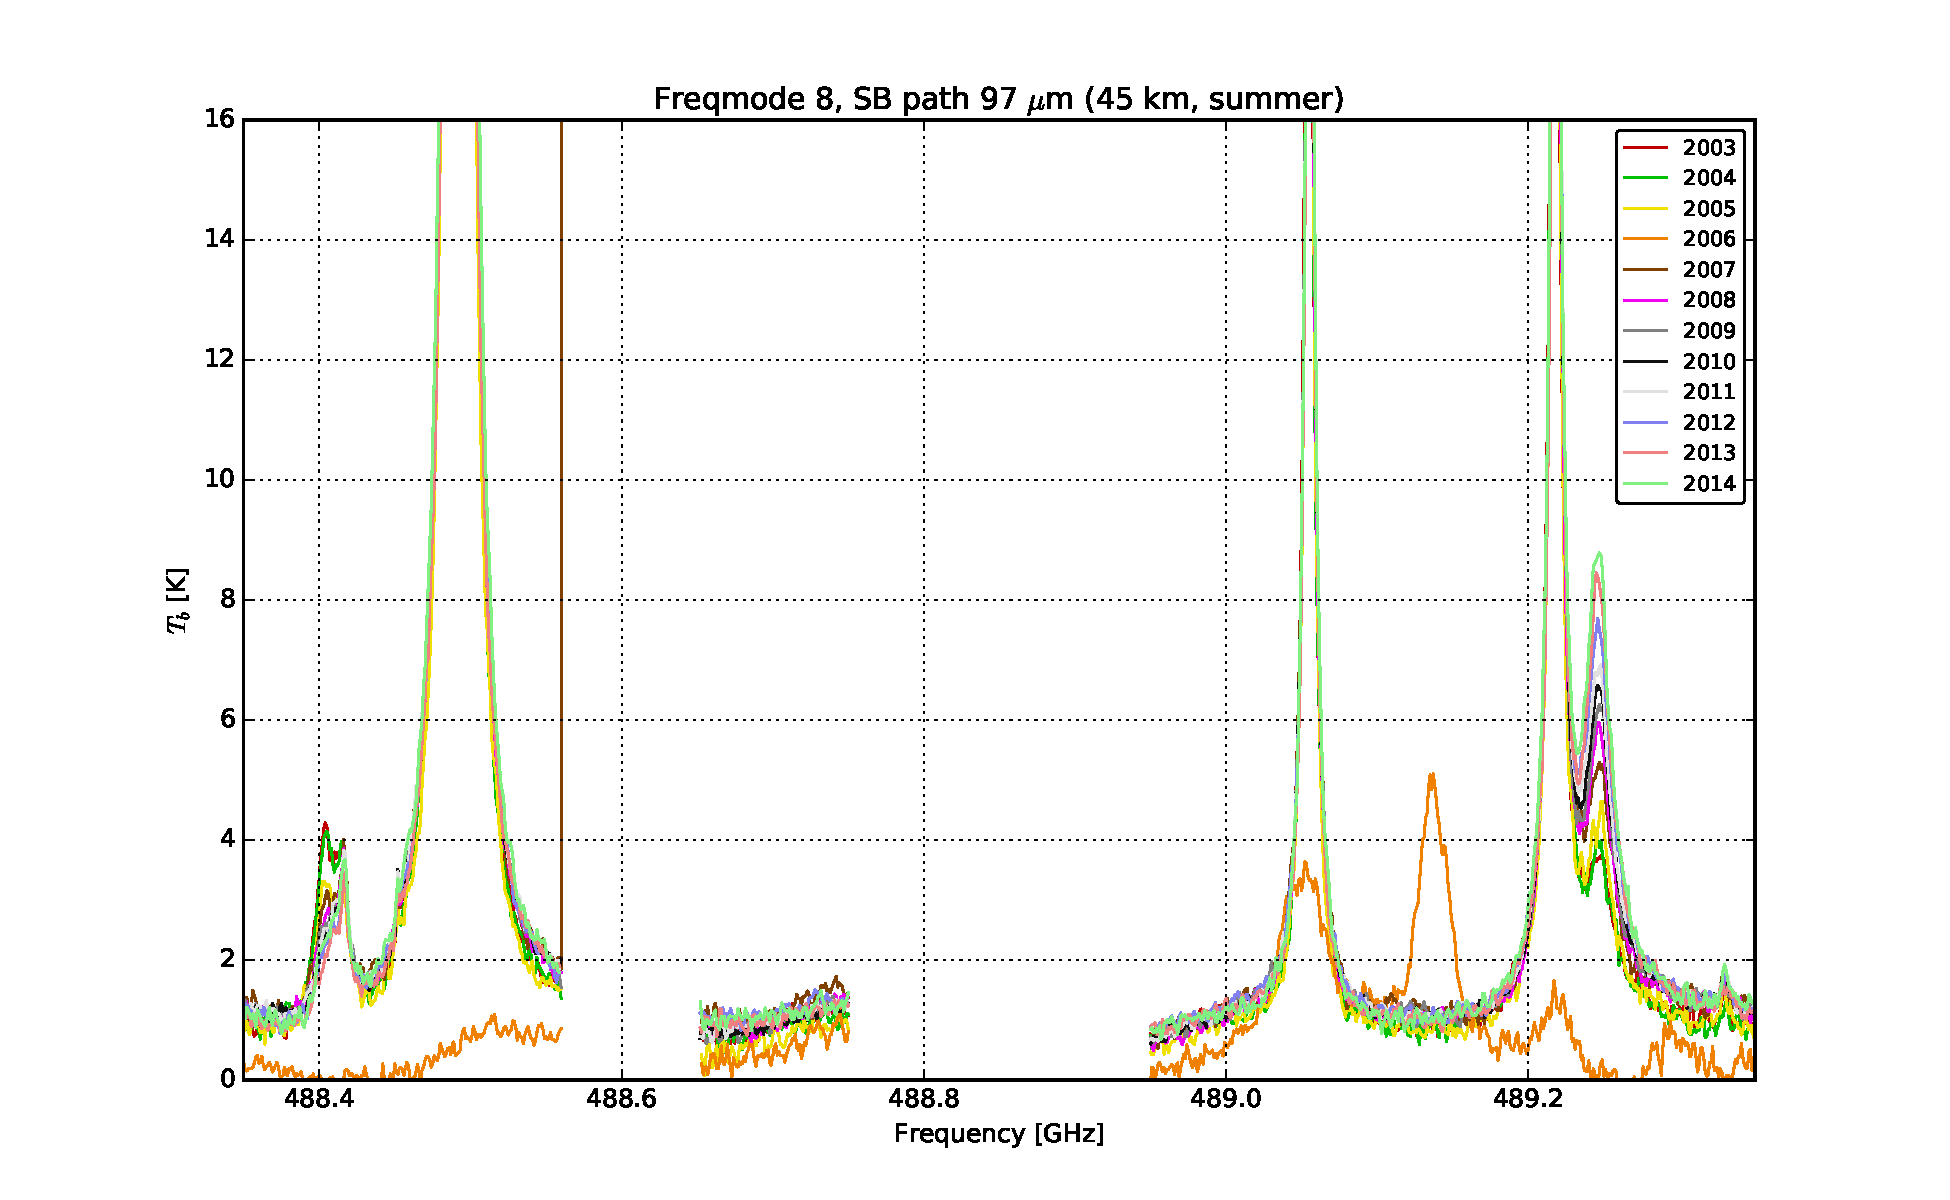
\includegraphics[width=\textwidth]{spectra/fm_08_spectra_summer_97u}
        \caption{summer}\label{fig:spectra:08:summer:97u}
    \end{subfigure}
    \begin{subfigure}[b]{0.9545\textwidth}
        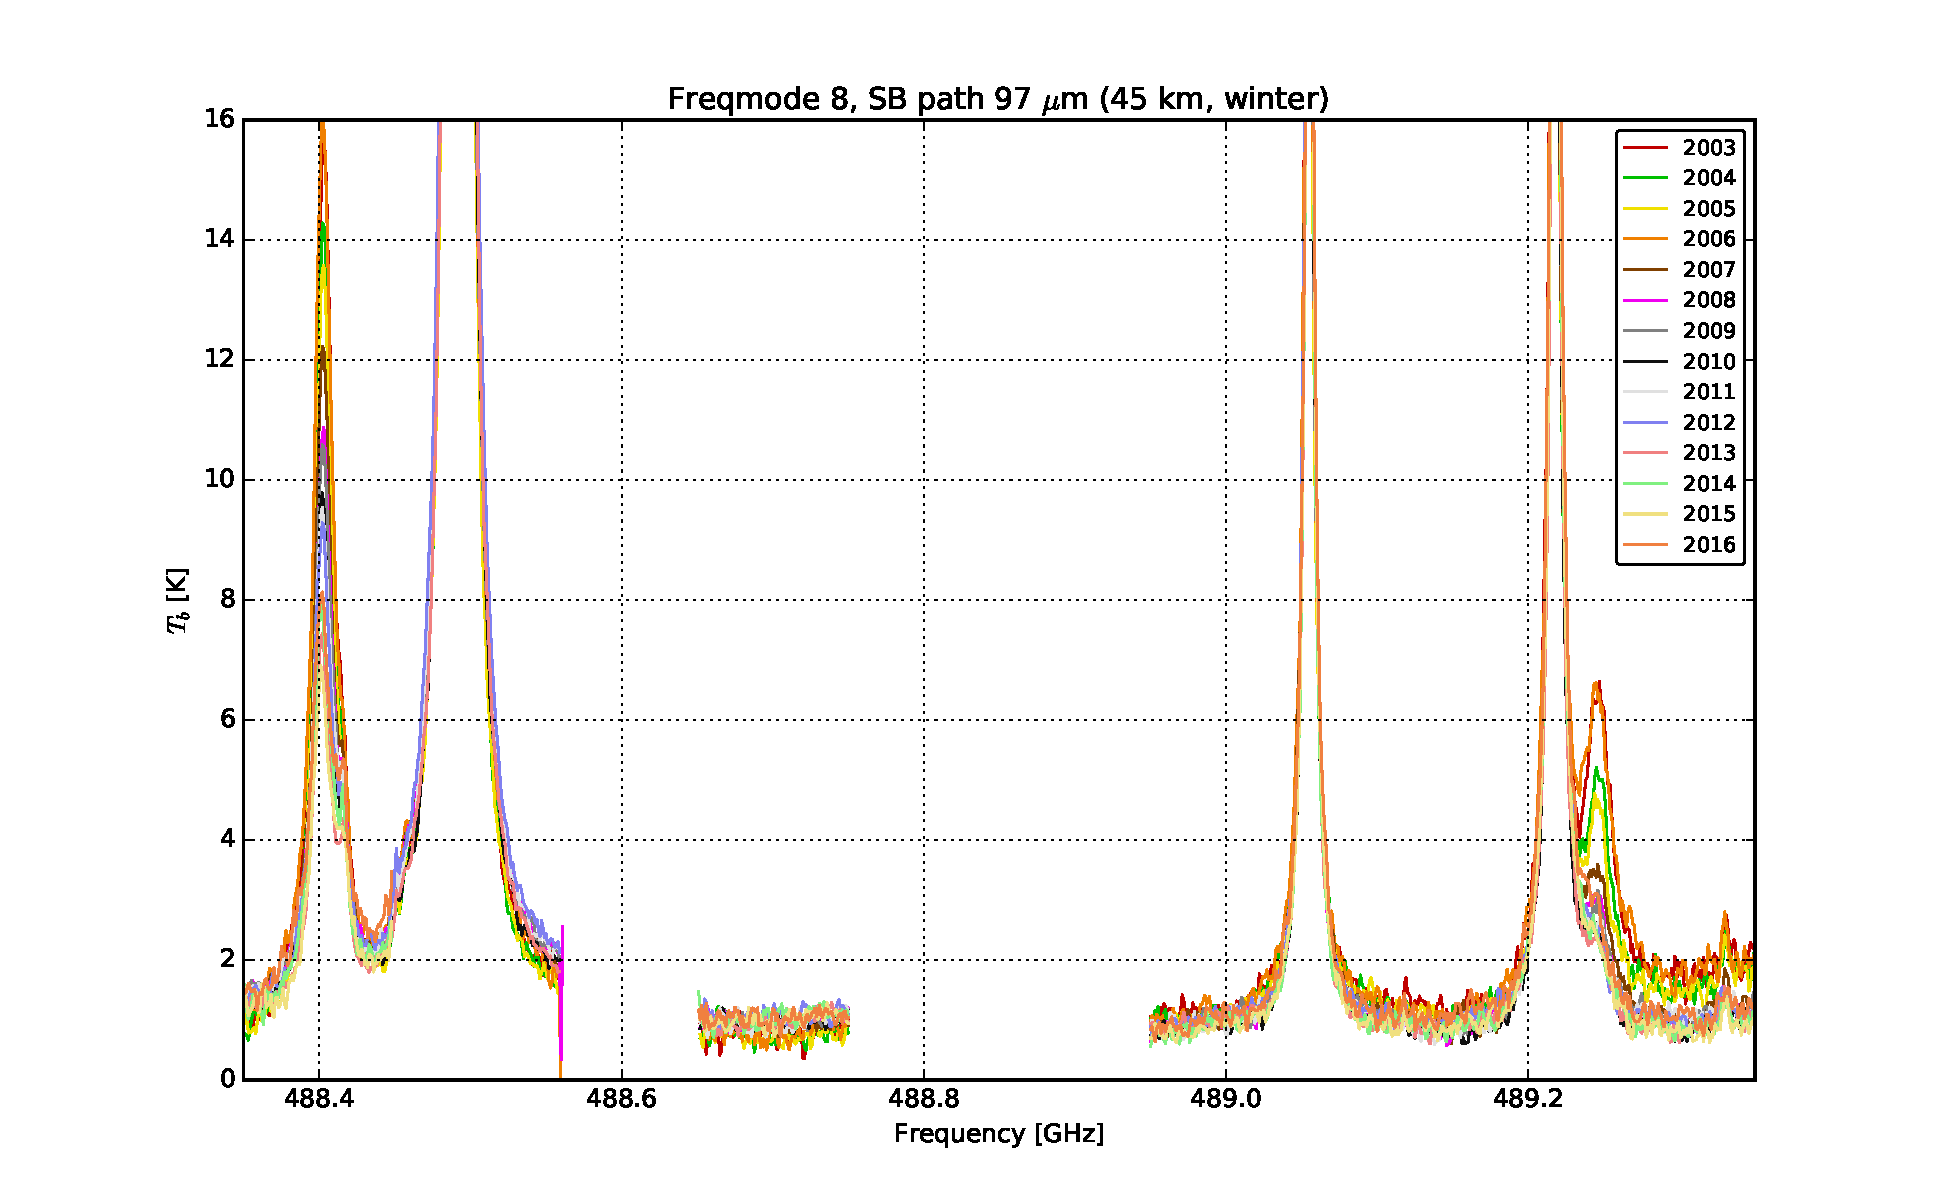
\includegraphics[width=\textwidth]{spectra/fm_08_spectra_winter_97u}
        \caption{winter}\label{fig:spectra:08:winter:97u}
    \end{subfigure}
    \caption{Annual median spectra for FM~08 for altitude interval 40--50~km at
        equatorial latitudes for the $97\,\mathrm{\mu m}$ sideband path. The
        unhealthy sub-bands~7 and~3 are between $\sim488.45$
        and~$488.65\,\mathrm{GHz}$.
        }\label{fig:spectra:08:97u}
\end{figure}

\begin{figure}[ht]
    \centering
    \begin{subfigure}[b]{0.9545\textwidth}
        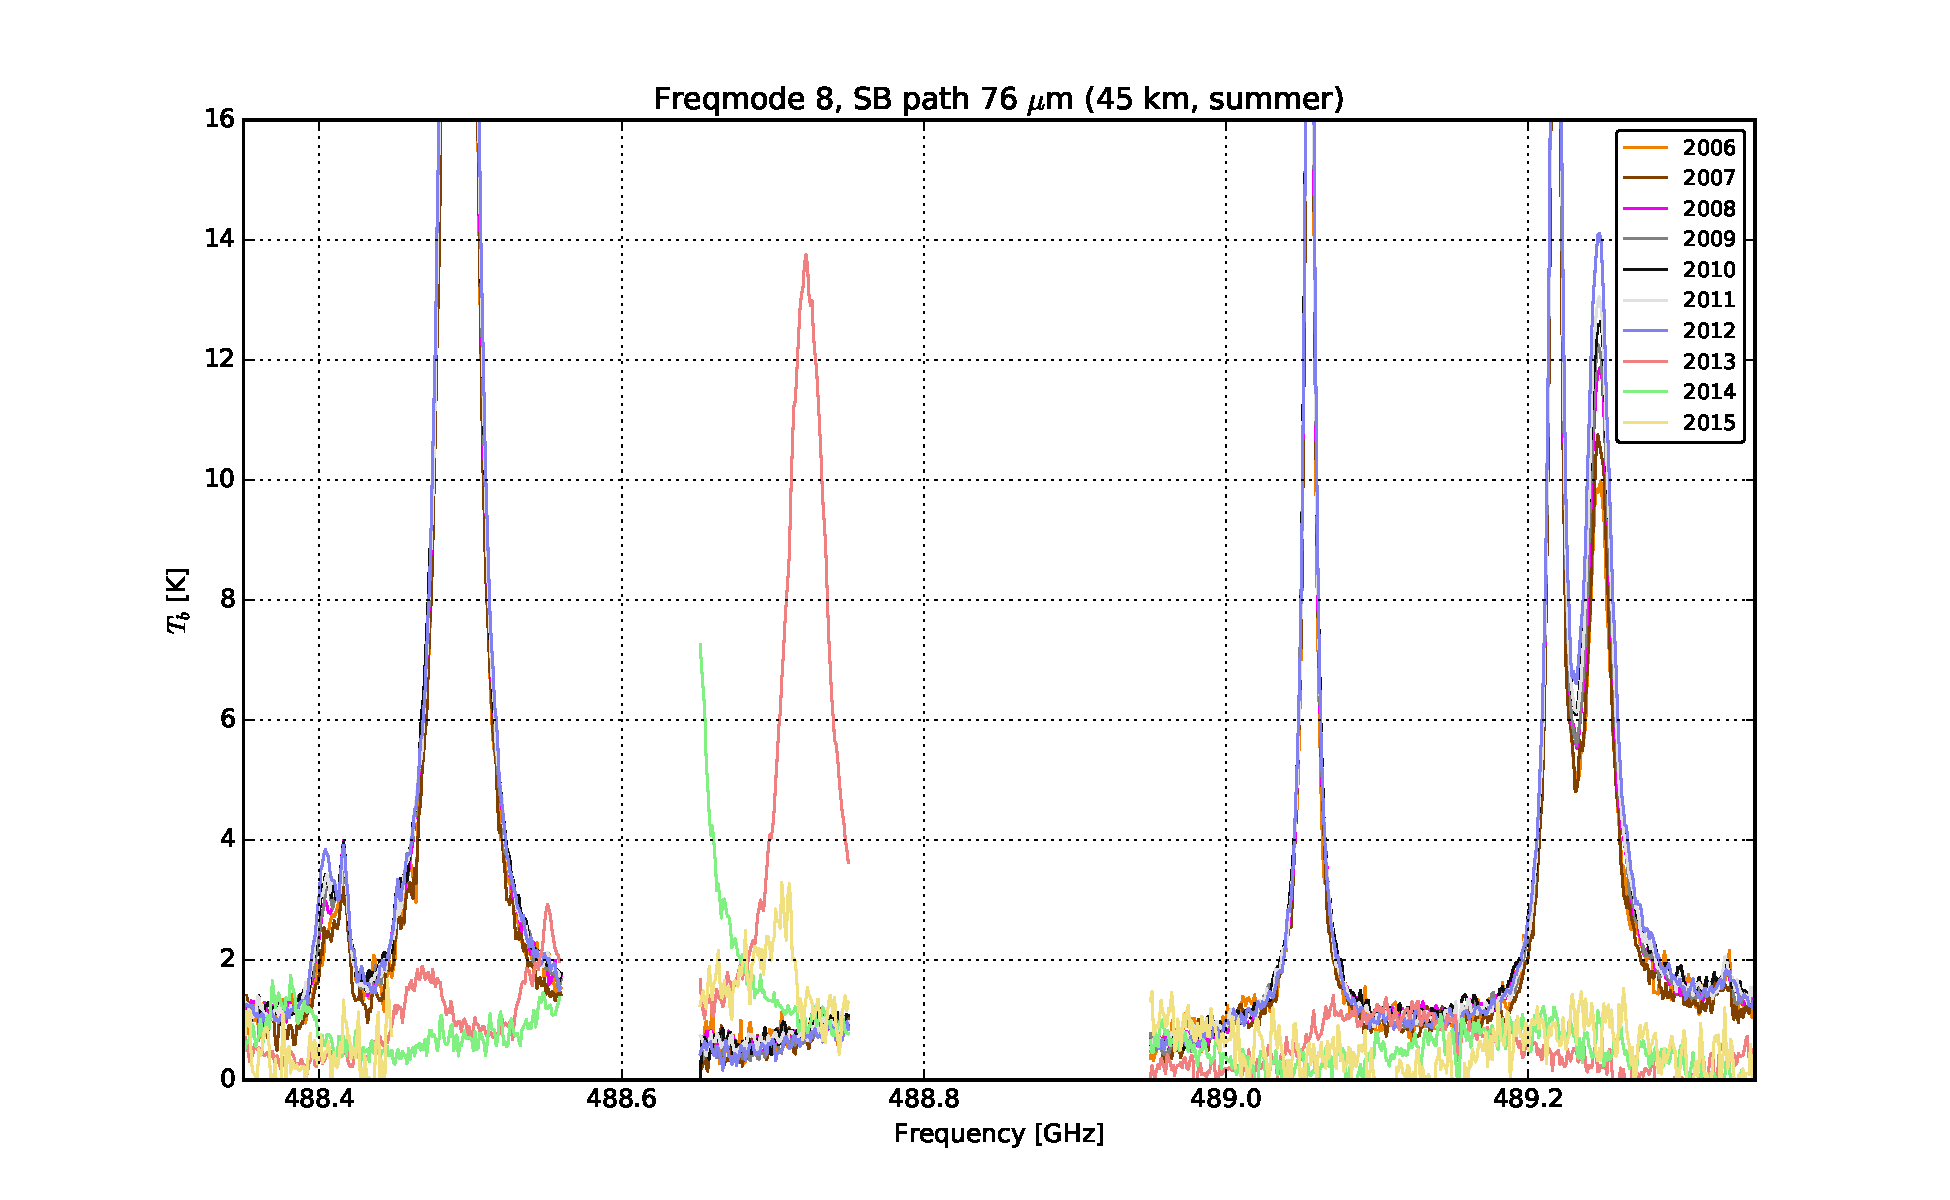
\includegraphics[width=\textwidth]{spectra/fm_08_spectra_summer_76u}
        \caption{summer}\label{fig:spectra:08:summer:76u}
    \end{subfigure}
    \begin{subfigure}[b]{0.9545\textwidth}
        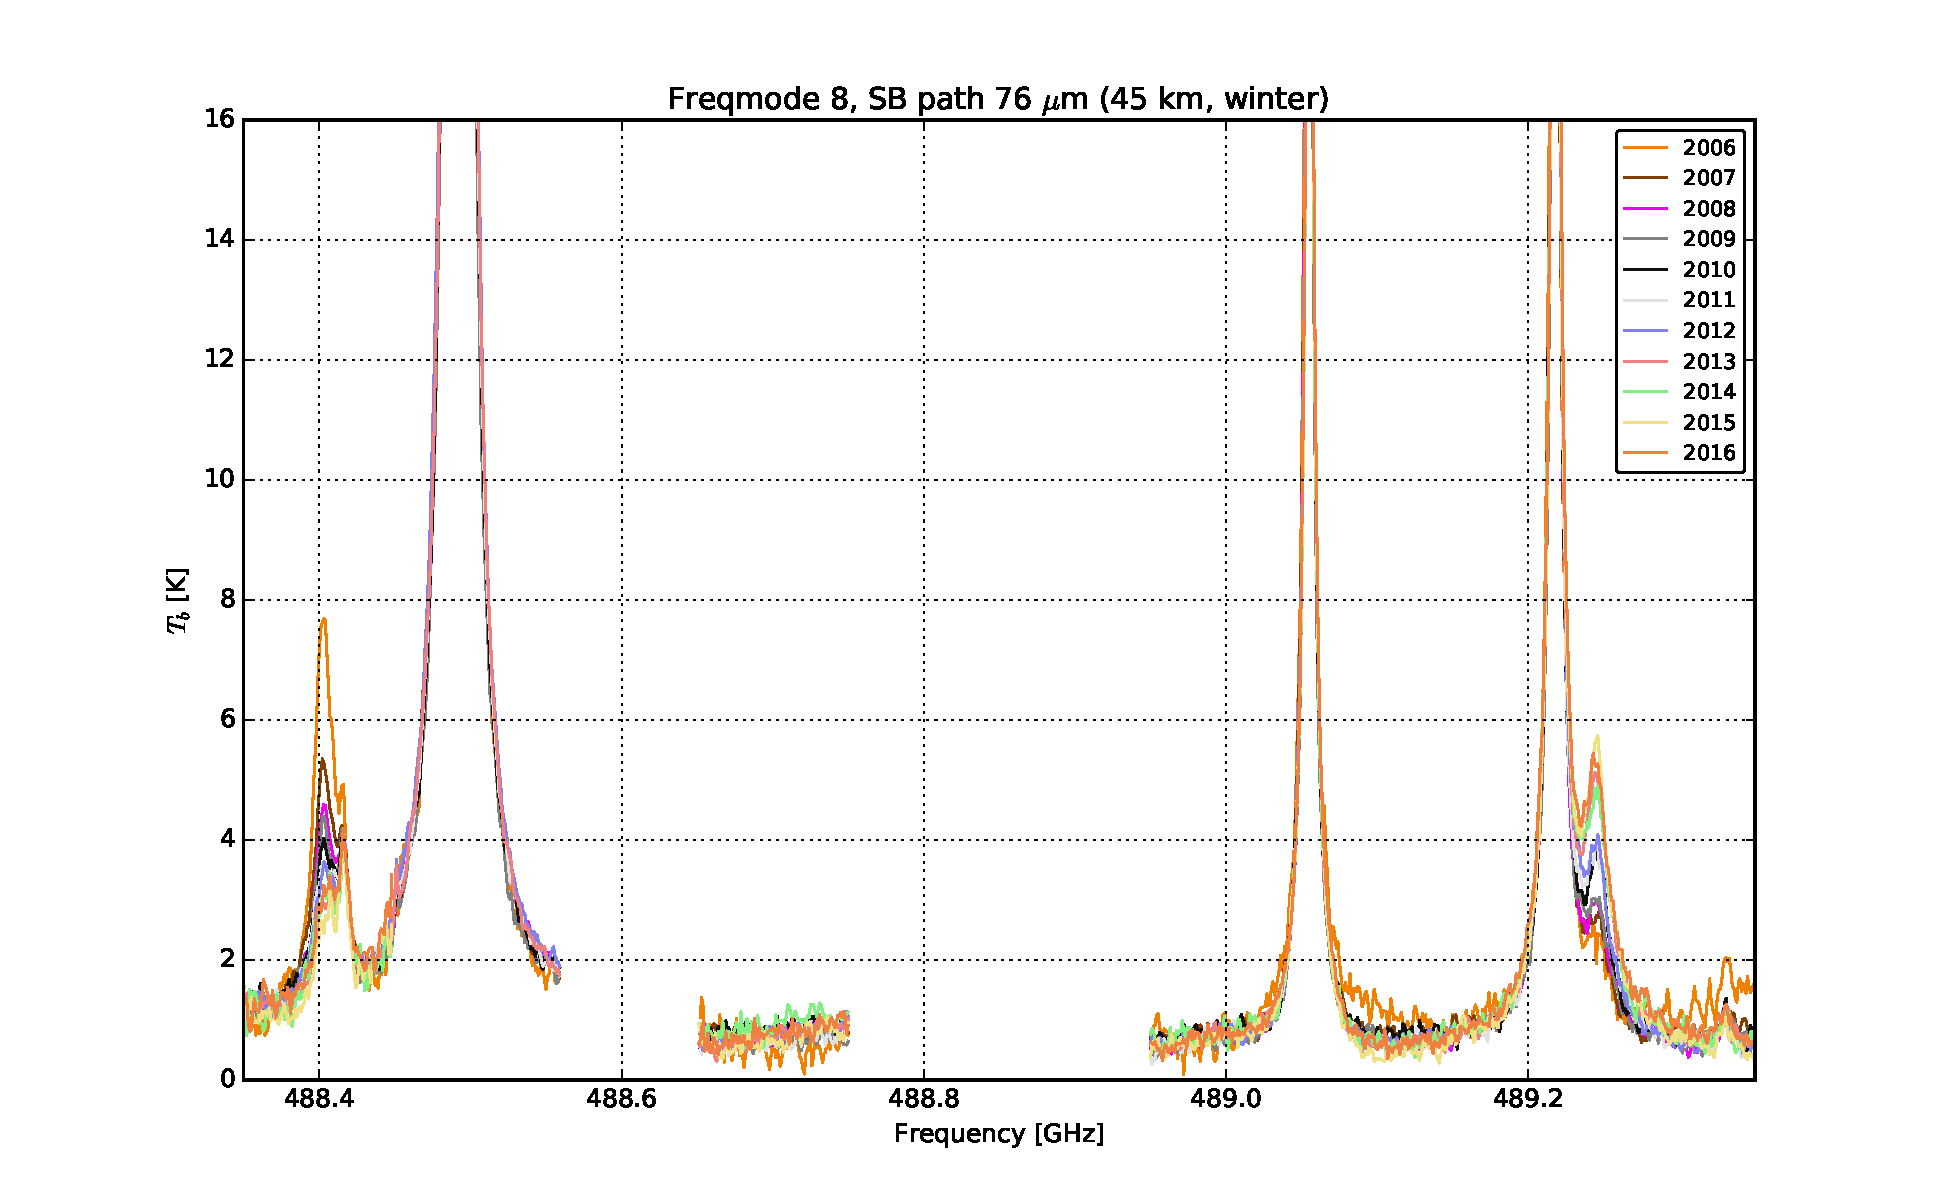
\includegraphics[width=\textwidth]{spectra/fm_08_spectra_winter_76u}
        \caption{winter}\label{fig:spectra:08:winter:76u}
    \end{subfigure}
    \caption{Annual median spectra for FM~08 for altitude interval 40--50~km at
        equatorial latitudes for the $76\,\mathrm{\mu m}$ sideband path. The
        unhealthy sub-bands~7 and~3 are between $\sim488.45$
        and~$488.65\,\mathrm{GHz}$.
        }\label{fig:spectra:08:76u}
\end{figure}

\begin{figure}[ht]
    \centering
    \begin{subfigure}[b]{0.9545\textwidth}
        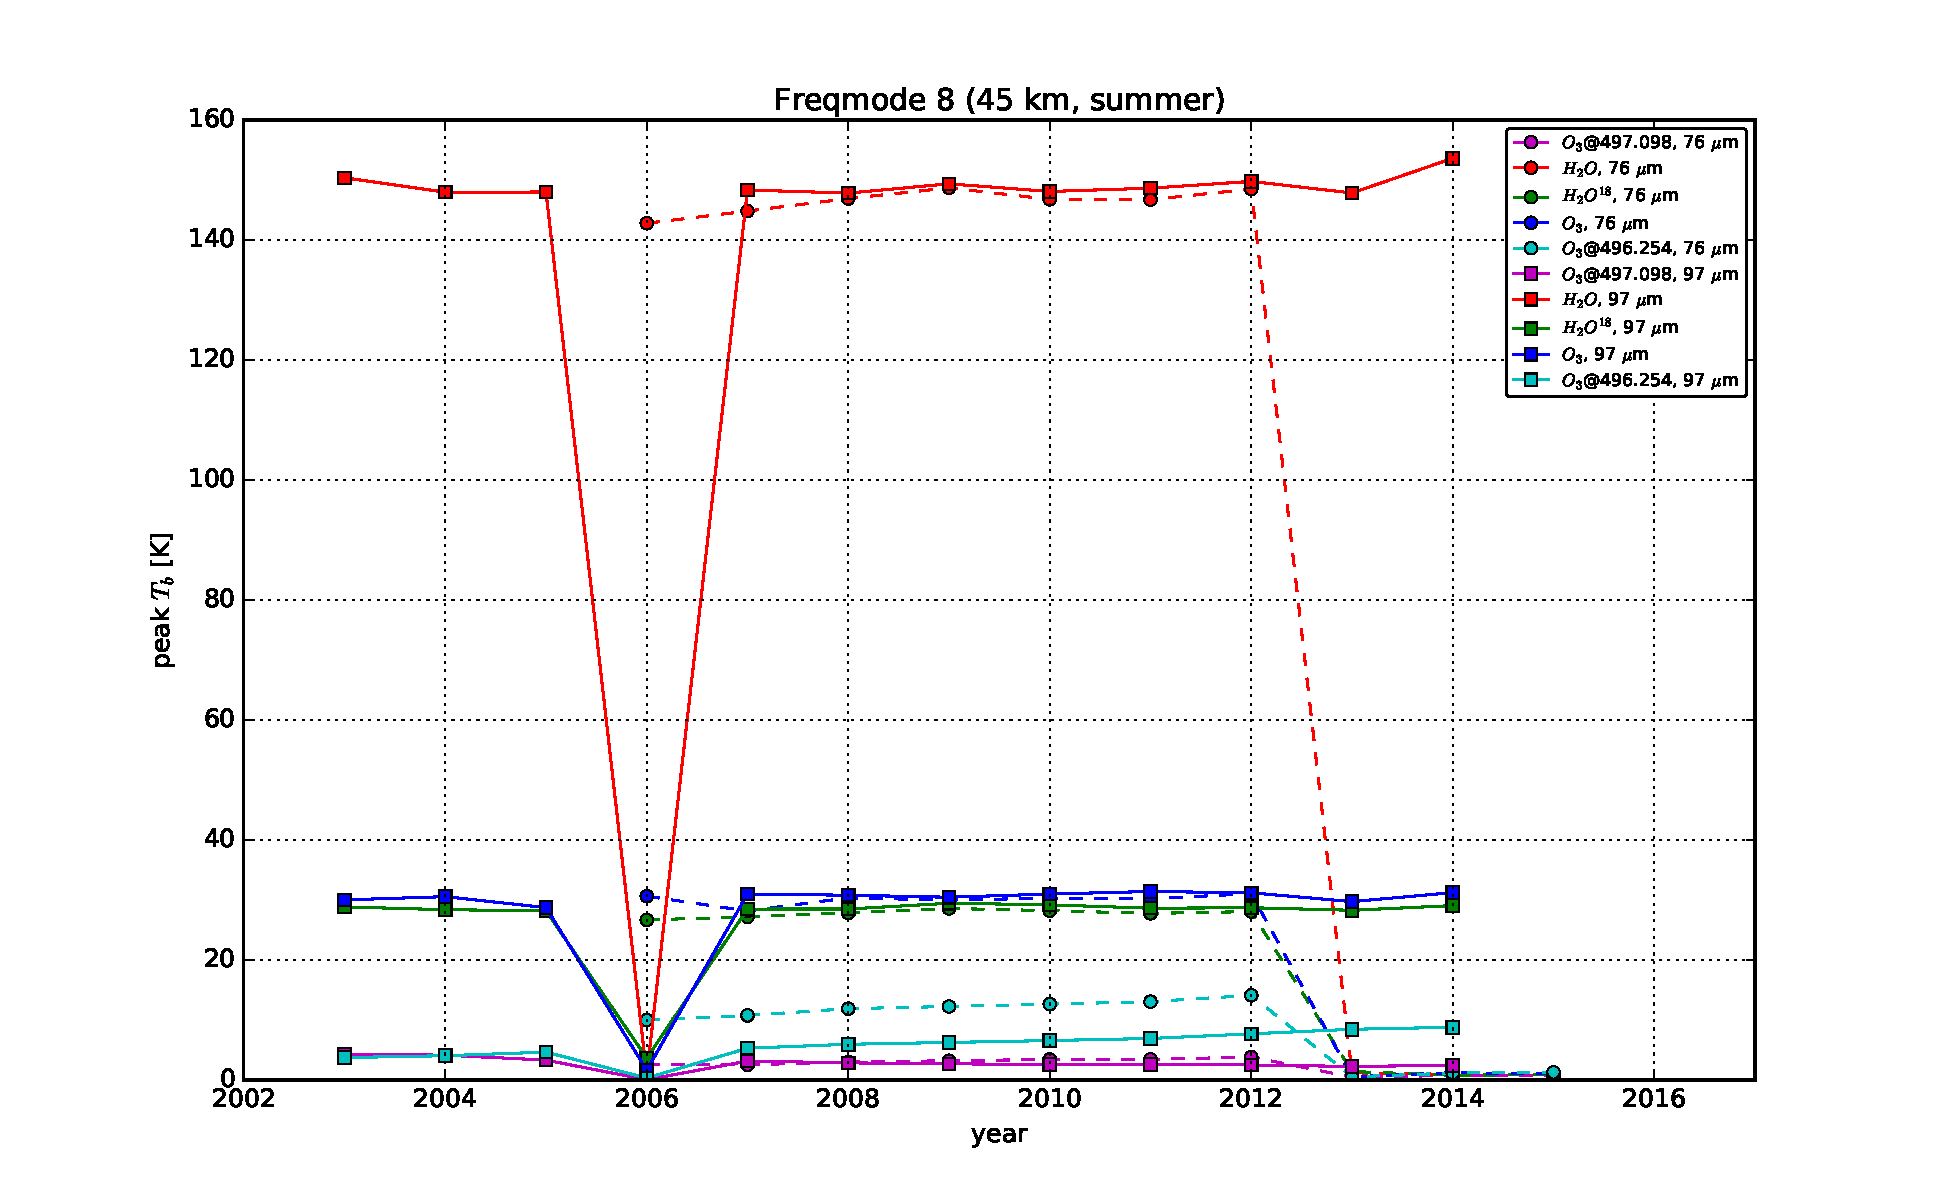
\includegraphics[width=\textwidth]{peaks/fm_08_peaks_summer}
        \caption{summer}\label{fig:peaks:08:summer}
    \end{subfigure}
    \begin{subfigure}[b]{0.9545\textwidth}
        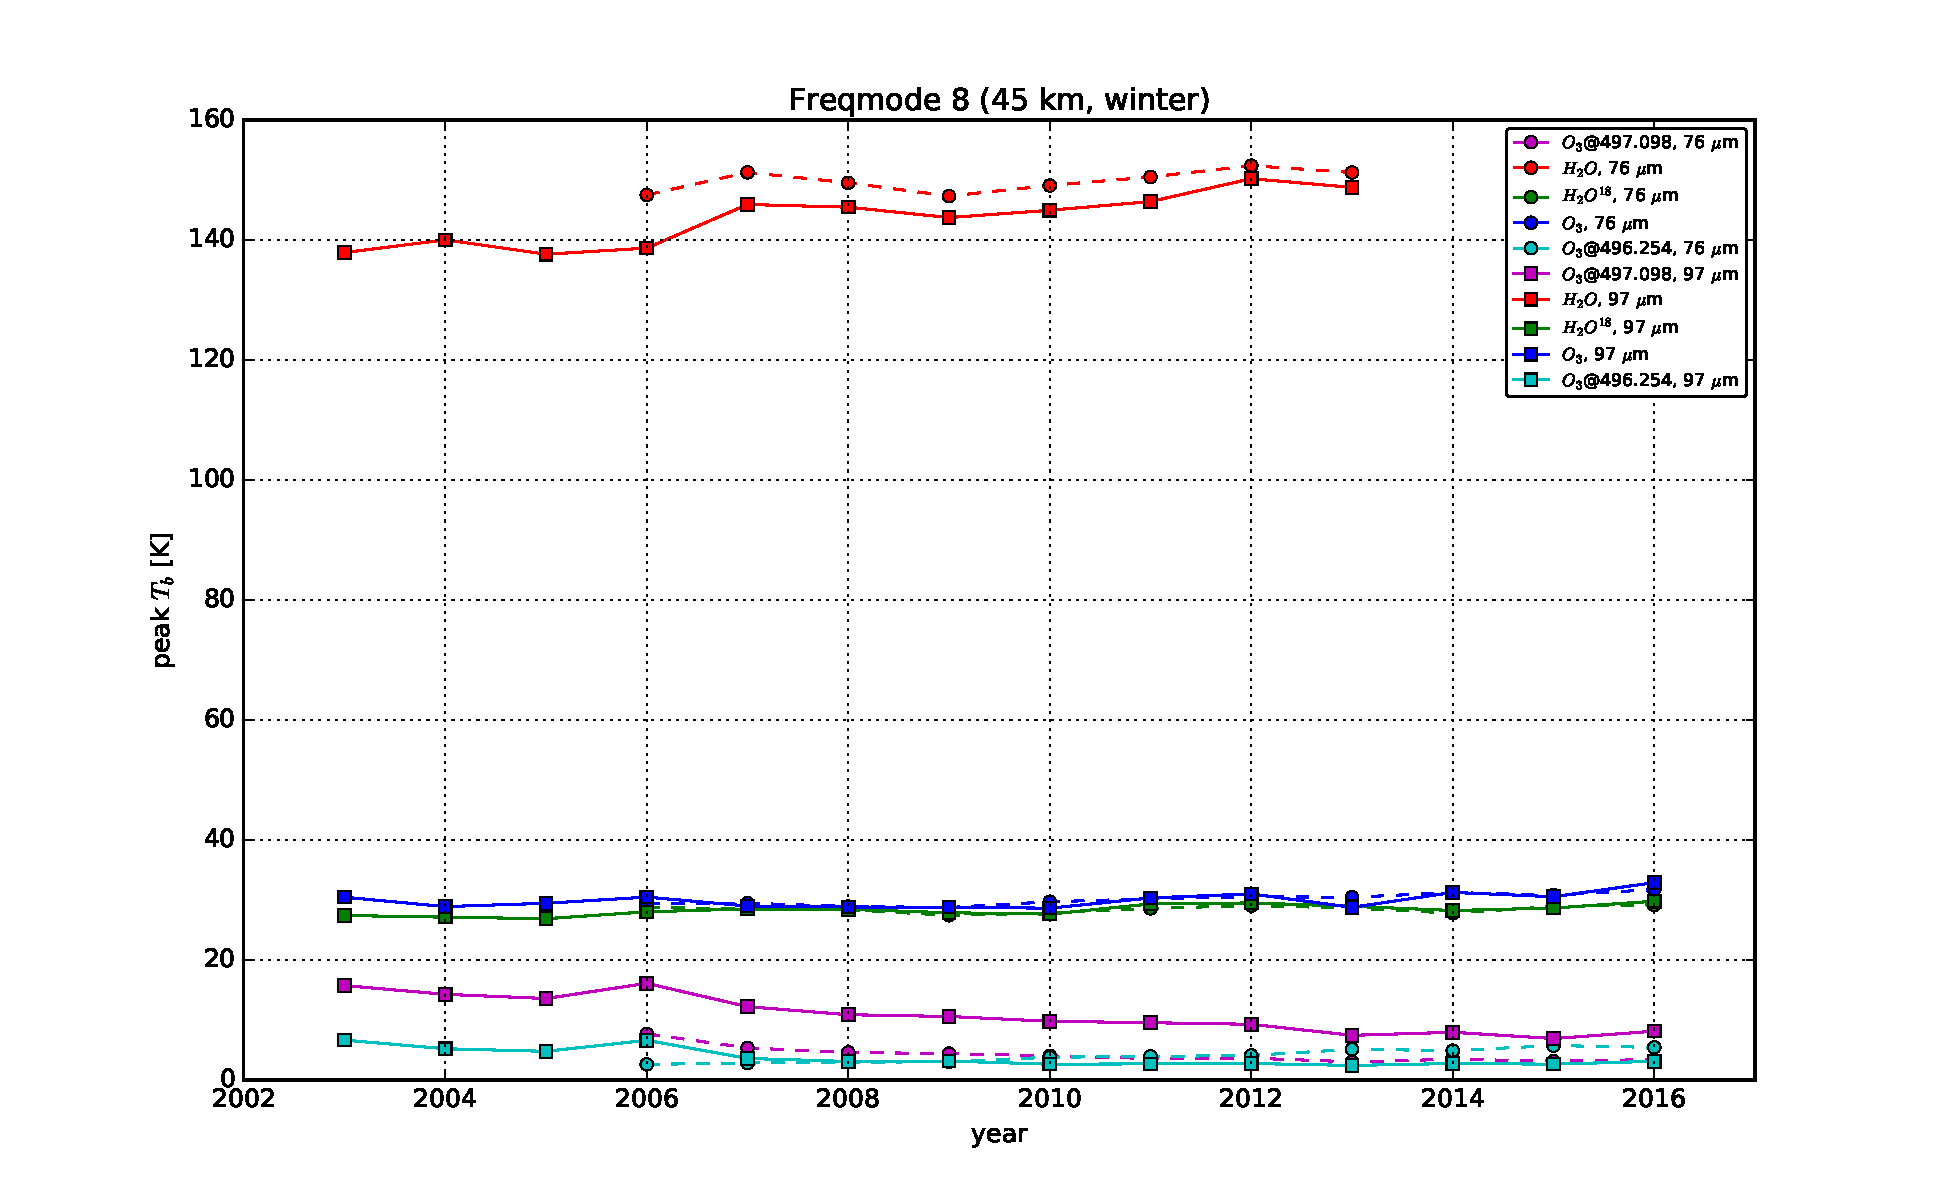
\includegraphics[width=\textwidth]{peaks/fm_08_peaks_winter}
        \caption{winter}\label{fig:peaks:08:winter}
    \end{subfigure}
    \caption{Annual median peak values for FM~08 for altitude interval
        40--50~km at equatorial latitudes for both sideband paths.
        Values extracted for the the \chem{H_2O} peak
        at~$\sim488.494\,\mathrm{GHz}$, the \chem{H_2O^{18}} peak
        at~$\sim489.055\,\mathrm{GHz}$, the \chem{O_3} peak
        at~$\sim489.218\,\mathrm{GHz}$, and the \chem{O_3} sideband peaks
        at~$\sim488.405$ and $\sim489.247\,\mathrm{GHz}$,
        in Figs.~\ref{fig:spectra:08:97u} and~\ref{fig:spectra:08:76u}.
        }\label{fig:peaks:08}
\end{figure}

\noindent
FM~08 is different from the other modes in two respects: first, it is a lower
sideband mode, which for the purpose of this report is not important; second,
it has utilised two separate sideband paths for most of its operation, that
show distictly different sideband leakage charateristics.  Yearly median
spectra for summer and winter at $\sim45\,\mathrm{km}$ are shown in
Figs.~\ref{fig:spectra:08:97u} and~\ref{fig:spectra:08:76u} for the two
sideband paths~$97$ and~$76\,\mathrm{\mu m}$ respectively, and the trend over
time of the different peaks can be seen in Fig.~\ref{fig:peaks:08}.

It is evident from the pictures that the sideband peaks (far left and far right
in the figures) have changed over the years, but the trends are different both
depending on which sideband path is looked at, and depending on the season.
These issues are discussed in greater detail in Sec.~\ref{FM08:sbl} below.
Apart from the sideband issues, and apart from a glitch in the summer of 2006
the spectra for the $97\,\mathrm{\mu m}$ path look good for both seasons.
Likewise, the spectra for the $76\,\mathrm{\mu m}$ also look good for both
seasons, apart from the summers of 2013--2016, in the last of which the this
path was not used at all.


\subsection{Sideband leakage}
\label{FM08:sbl}

\begin{figure}[ht]
    \centering
    \begin{subfigure}[b]{0.9545\textwidth}
        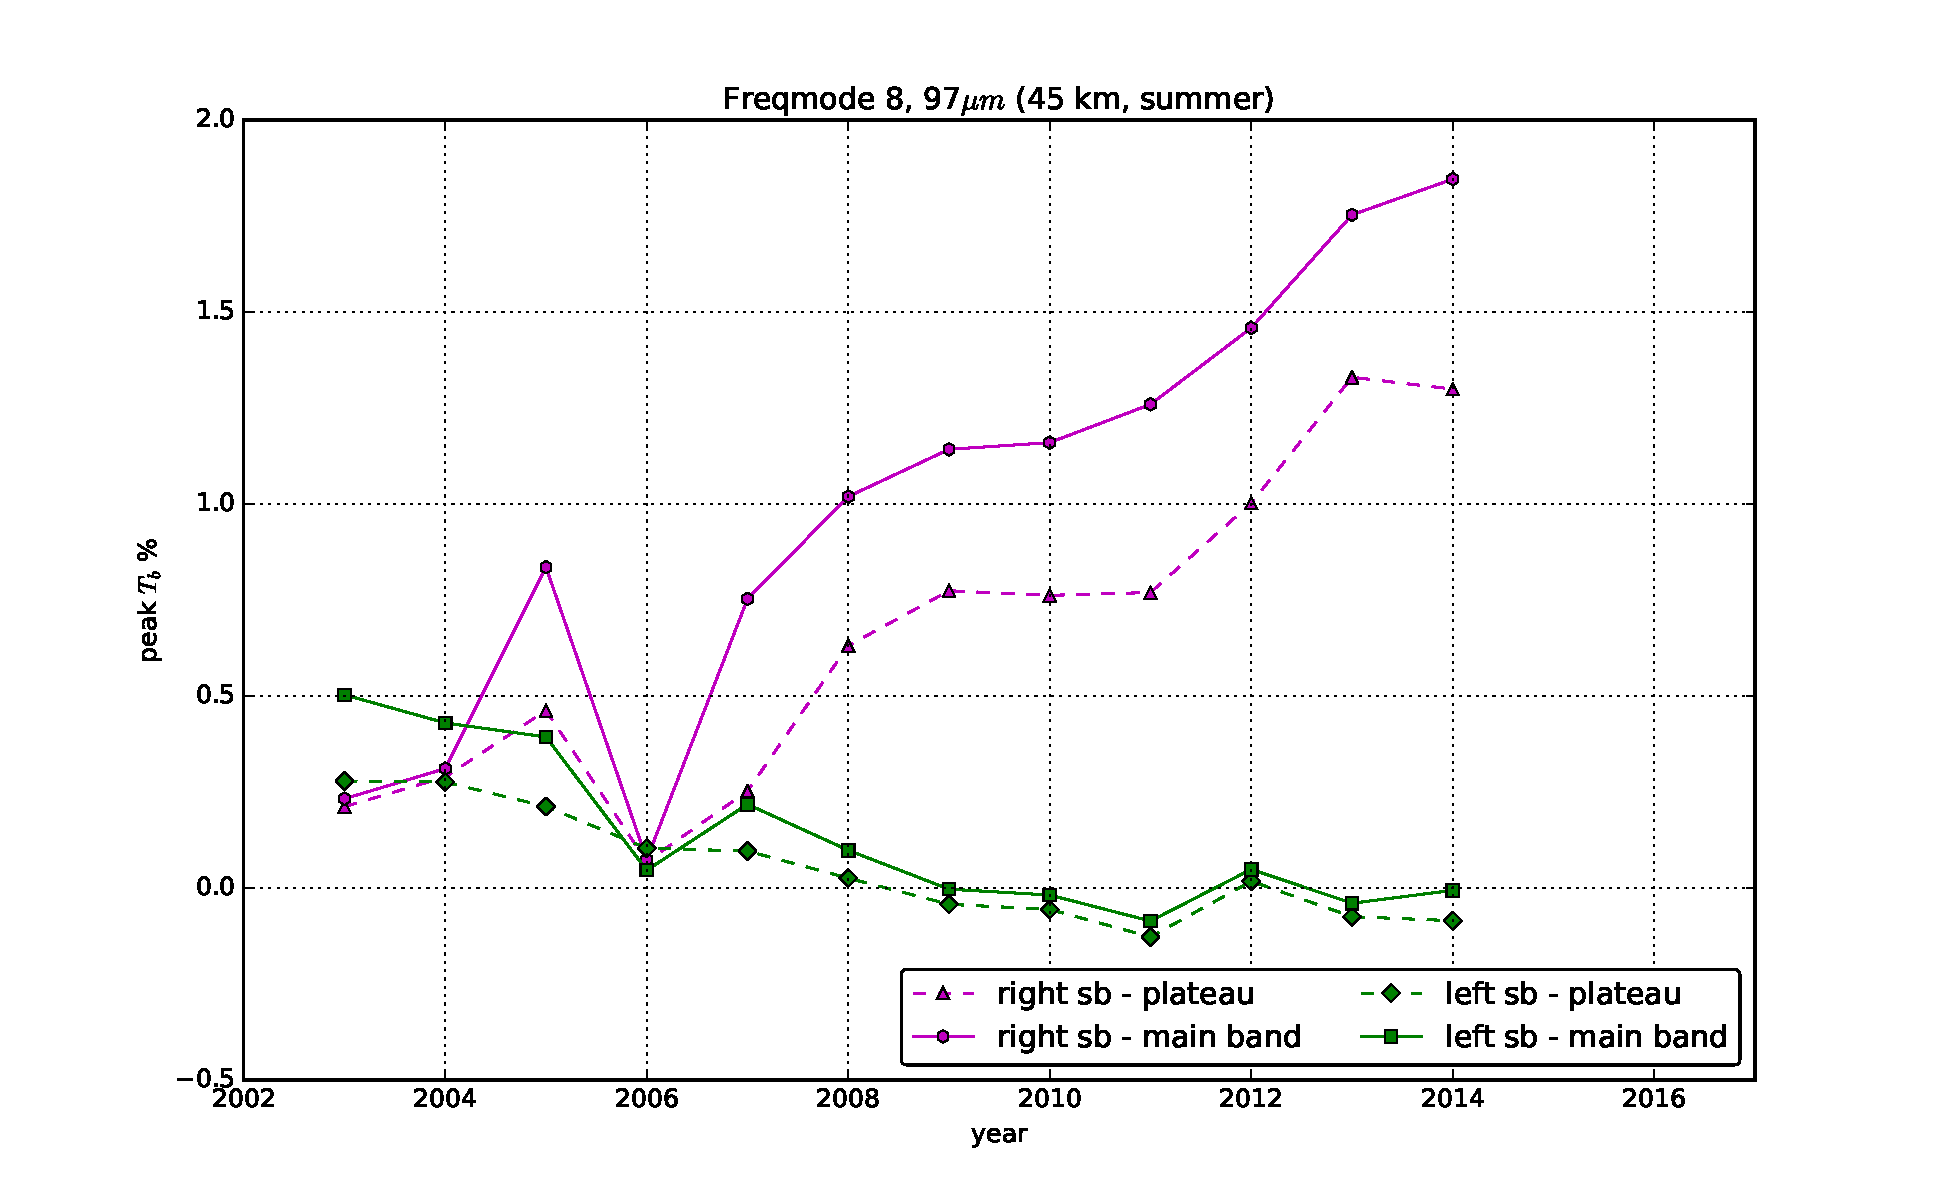
\includegraphics[width=\textwidth]{peaks/fm_08_sbl_summer_97u}
        \caption{summer}\label{fig:sbl:08:summer:97u}
    \end{subfigure}
    \begin{subfigure}[b]{0.9545\textwidth}
        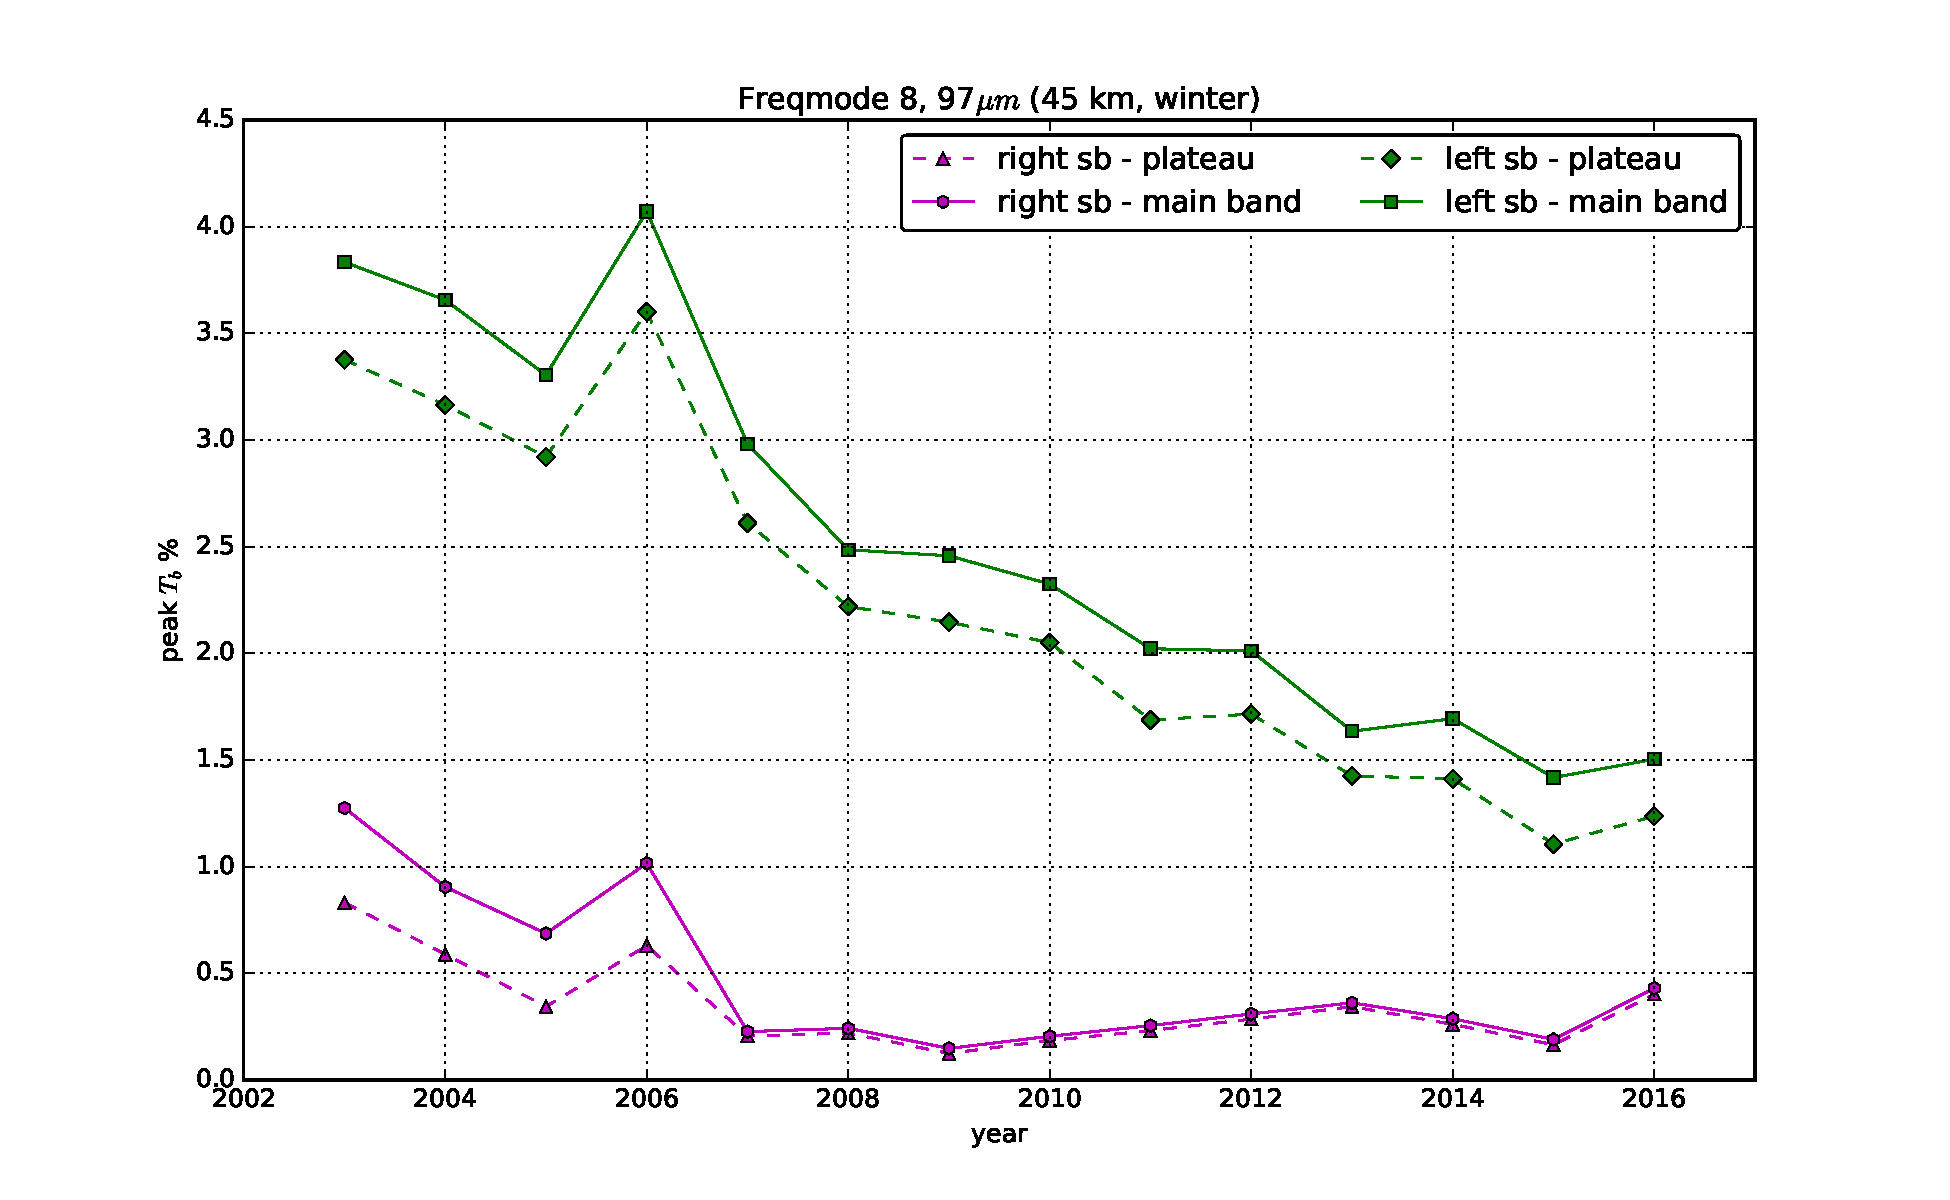
\includegraphics[width=\textwidth]{peaks/fm_08_sbl_winter_97u}
        \caption{winter}\label{fig:sbl:08:winter:97u}
    \end{subfigure}
    \caption{Sideband leakages in \% calculated from the data shown in
        Fig.~\ref{fig:spectra:08:97u} for the $97\,\mathrm{\mu m}$ sideband
        path.  Values were calculated by subtracting the value of the
        ``plateau'' on the side of each sideband peaks nearest its
        neighbouring main band peak, or a first order approximation of the
        main band value under the peak.  The results were compared with~$245.5$
        and~$256.8\,\mathrm{K}$ for the left and right sideband peaks
        respectively, values deemed representative of the actual peak
        intensities.
        }\label{fig:sbl:08:97u}
\end{figure}

\begin{figure}[ht]
    \centering
    \begin{subfigure}[b]{0.9545\textwidth}
        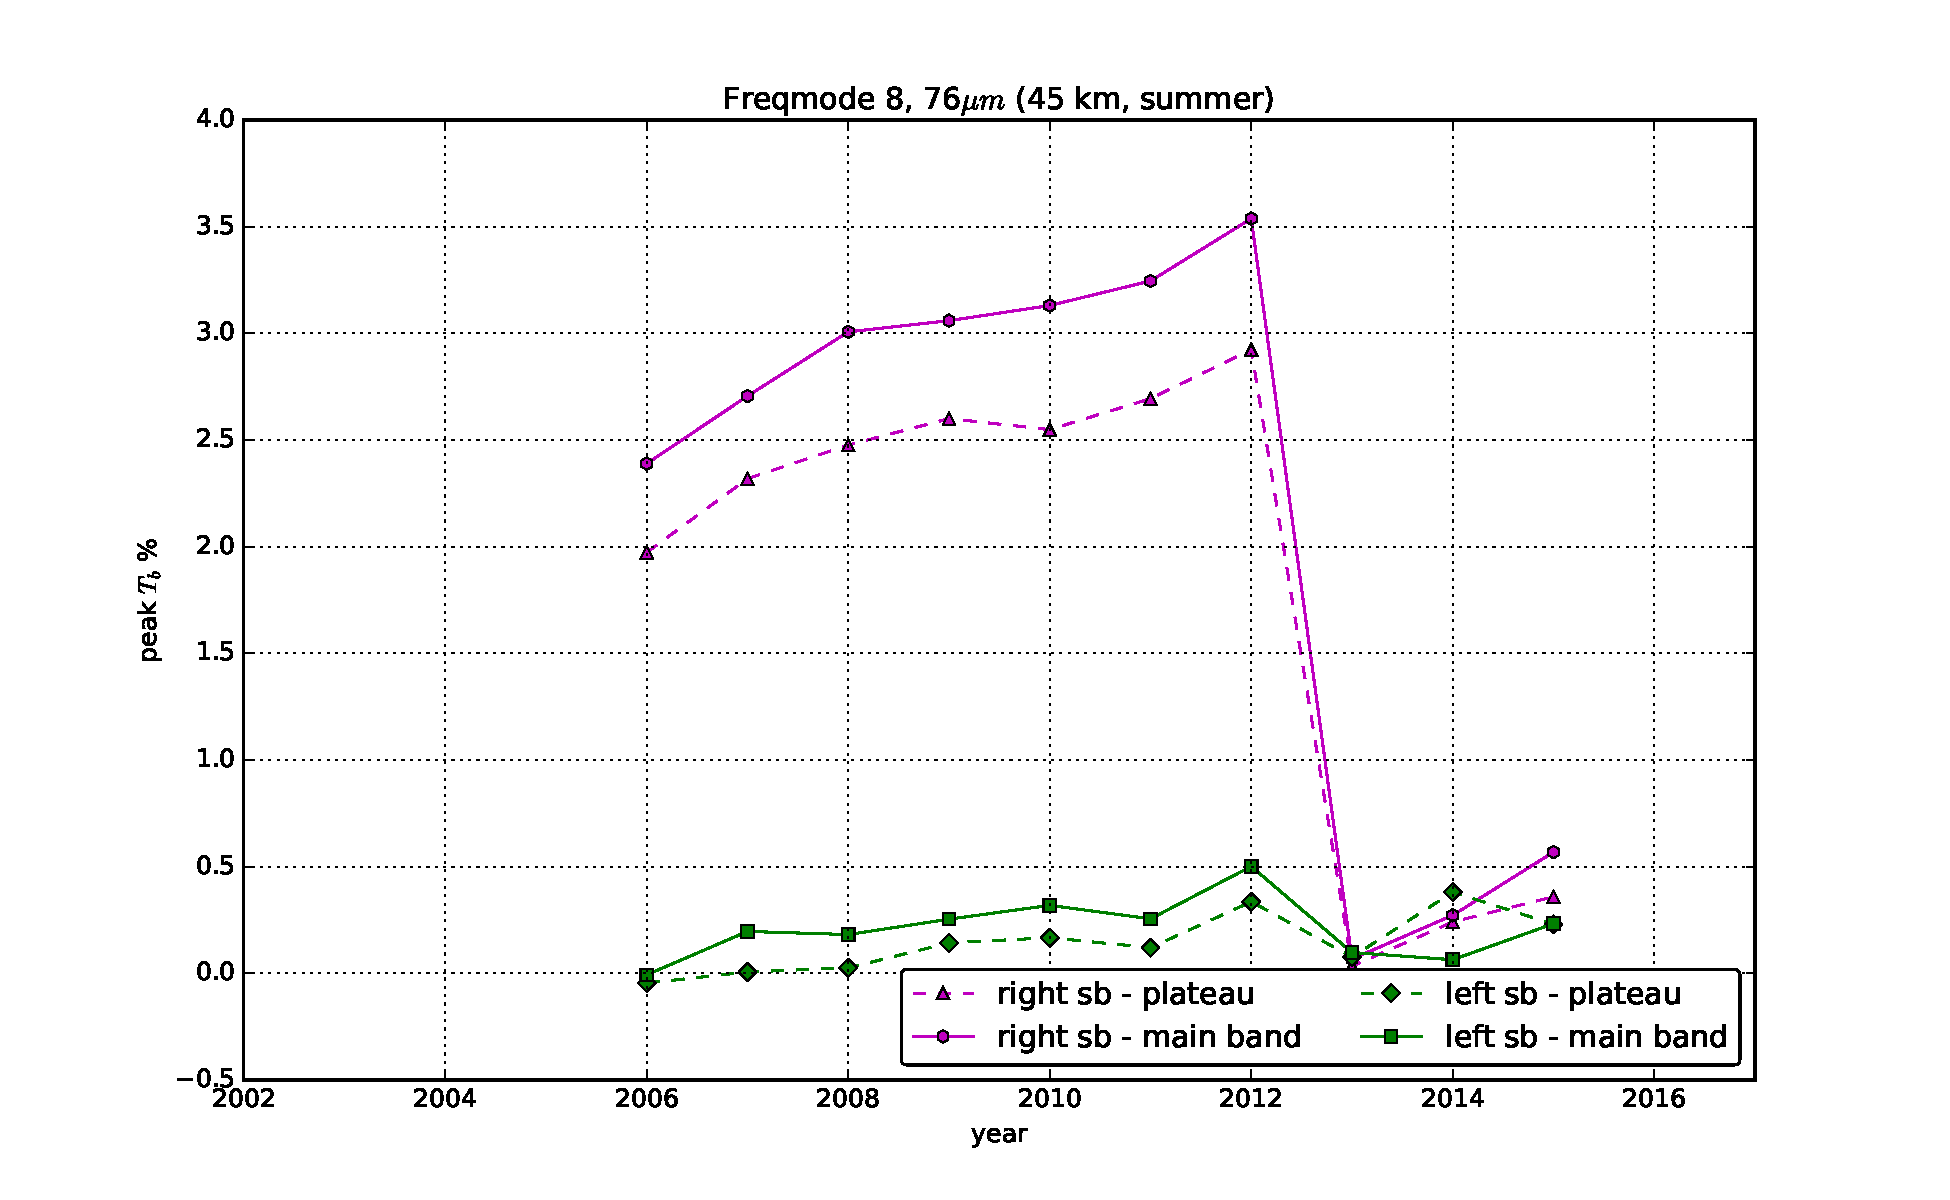
\includegraphics[width=\textwidth]{peaks/fm_08_sbl_summer_76u}
        \caption{summer}\label{fig:sbl:08:summer:76u}
    \end{subfigure}
    \begin{subfigure}[b]{0.9545\textwidth}
        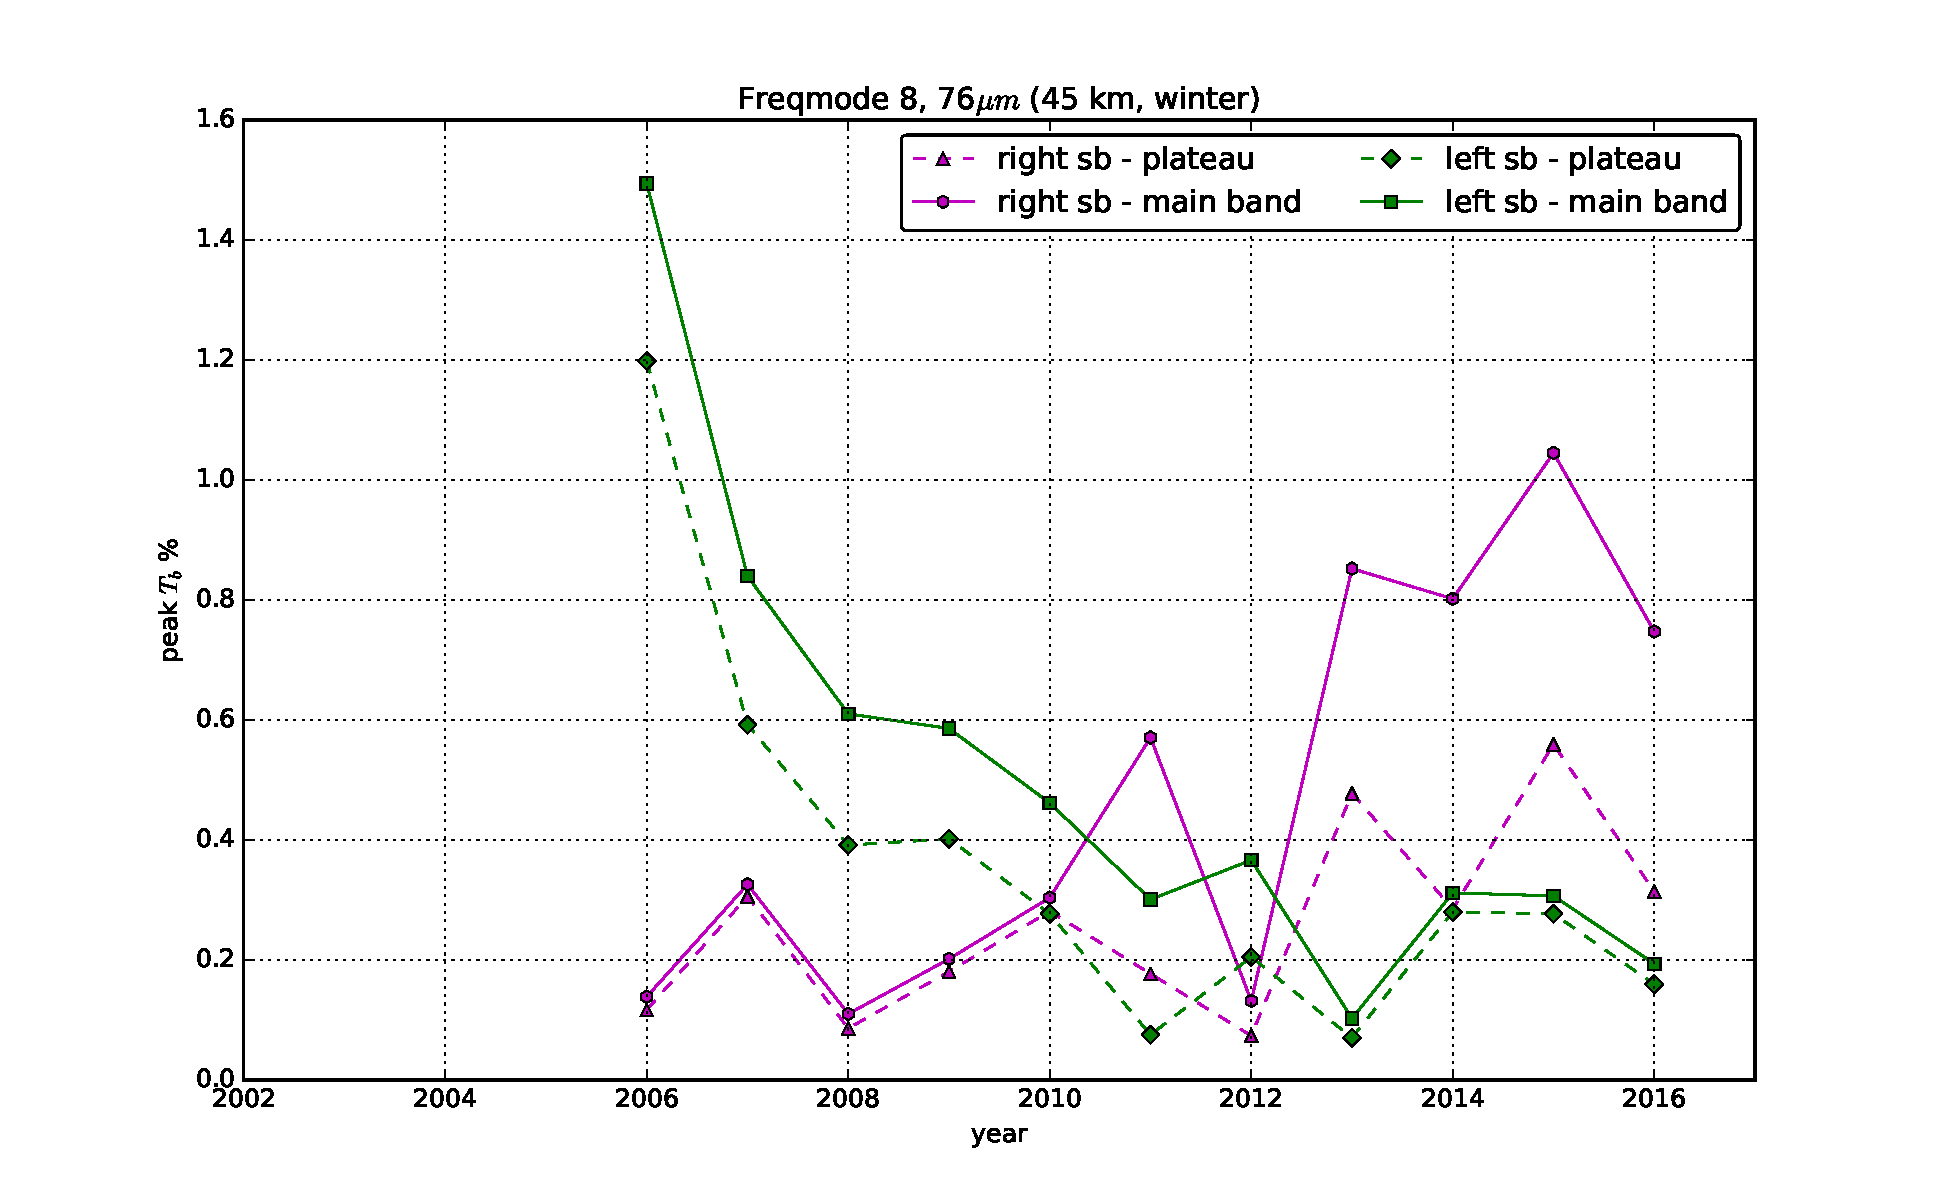
\includegraphics[width=\textwidth]{peaks/fm_08_sbl_winter_76u}
        \caption{winter}\label{fig:sbl:08:winter:76u}
    \end{subfigure}
    \caption{Sideband leakages in \% calculated from the data shown in
        Fig.~\ref{fig:spectra:08:76u} for the $76\,\mathrm{\mu m}$ sideband
        path.  Values were calculated by subtracting the value of the
        ``plateau'' on the side of each sideband peaks nearest its
        neighbouring main band peak, or a first order approximation of the
        main band value under the peak.  The results were compared with~$245.5$
        and~$256.8\,\mathrm{K}$ for the left and right sideband peaks
        respectively, values deemed representative of the actual peak
        intensities.
        }\label{fig:sbl:08:76u}
\end{figure}

\noindent
The sideband leakage was estimated at $\sim45\,\mathrm{km}$ by taking the
sideband peak intensities from the data shown in Figs.~\ref{fig:spectra:08:97u}
and~\ref{fig:spectra:08:76u} and subtracing the main band intensities estimated
by two methods:  by taking the value of the ``plateau'' on the side of each
sideband peak nearest its neighbouring main band peak as the main band value, and
by making first order approximation of the value directly under the peak.  The
actual value should between these two estimates, but closer to the latter.

To estimate the leakage, the extracted peak intensities were then divided by an
expected sideband peak intensity from simulations using
ARTS~(\cite{buehler:artst:05}).  $245.5$~and $256.8\,\mathrm{K}$ were chosen as
representative values for the left and right sideband peaks respectively, but
the peak values vary by $\sim2\,\mathrm{K}$ from year to year.  The results are
shown in Figs.~\ref{fig:sbl:08:97u} and~\ref{fig:sbl:08:76u} where it can be
seen that the sideband leakage varies differently over time for the two peaks
and furthermore, that the variation is different both depending on sideband
path and season.  These matters are discussed in more detail below.  On the
whole, however, the sideband leakage seems to be comparatively small for this
particular frequency mode, with strictly less than $5\%$ leakage and typically
less than $2\%$.  It should be noted, that even if the supression seems to be
working within operational parameters, the effect of a higher leakage is still
very large, since the sideband peaks have very high intensities.


\subsubsection{Sideband paths and seasonality}
\label{FM08:sbpath}
\label{FM08:seasonality}
The sideband filter for FM~08 uses two more or less distinct values for the
sideband path length in equal measure: $97\,\mathrm{\mu m}$ and
$76\,\mu\mathrm{m}$.  The leakage tendency varies for the two categories as
well as with season, and to confuse the matter even more, the trend is
different depending on which of the two strong peaks one is looking at.

As seen in Fig.~\ref{fig:sbl:08:97u}, for the $97\,\mathrm{\mu m}$ path the
sideband peak to the left has shown a decreasing tendency (increased
suppression) over time for both summers and winters. For summers the
leakage has decreased from the mostly insignificant level of $\sim0.5\%$ to
being barely detectalbe after 2008\footnote{N.B.: the estimated sideband
leakage presented in the figures is not reliable below $\sim0.25\%$ or so
\label{fn:sblestimate}}. For winters, on the other hand, the leakage starts out
at a fairly high $\sim4\%$ and drops to $\sim2\%$. For the sideband peak on the
right the trends are different between summer and winter, with the leakage
rising steadily from $\sim0.25\%$ to $\sim2\%$ during the summers, while
falling from $\sim1.5\%$ to below $0.5\%$ during the
winters\footref{fn:sblestimate}.
The same analysis was also performed for the $76\,\mathrm{\mu m}$ path, as can
be seen in Fig.~\ref{fig:sb:08:76u}.  For this sideband path, the trends are
not the same as for the $97\,\mathrm{\mu m}$ path, with the sideband peak to
the left has showing a low but increasing tendency over time for the summers
from $\sim0.25$ to $\sim0.5\%$, but a decreasing tendency from $\sim1.5\%$ to
$\sim0.4\%$ during the winters\footref{fn:sblestimate}, rather than decreasing
for both seasons. For the sideband peak on the right the trends are instead the
same in both summers and winters, with the leakage
rising steadily from $\sim2\%$ to $\sim3.5\%$ during the summers, and from
from $\sim0.25\%$ to $\sim1\%$ during the winters\footref{fn:sblestimate}.

The assymetry of the changes in the sideband leakage, both with respect to
frequency and sideband path, suggests that the phenomenon is due to a
misalignment in the sideband supression.  The difference between summers (cold)
and winters (warm) suggests that the phenomenon may be temerpature dependent,
which may also account for at least some of the change over time; see
Sec.~\ref{sec:Tcal} for details.
